\chapter{\uppercase{Programació}}
% Testejar cosetes i poder treure algun screenshot (?, o l'screen shot no fa falta?
% Adjuntar codi, aquí o en annex
S'ha desenvolupat un programa per adquirir correctament les senyals analògiques, calcular la tensions i mostrar-les en un parell de gràfiques en una web. Es porta un comptatge de temps per tal d'efectuar les lectures de tensió de forma periòdica. El programa mostra la web al client si aquest es connecta a l'adreça IP del dispositiu pel port 80, en aquest cas.
\section{Organigrama}
L'organigrama de la Figura \ref{fig:organigrama} és una forma simplificada d'explicar la solució adoptada. A l'annex de programa figura el codi complet.


% fill=blue!20, 
\tikzstyle{decision} = [diamond, draw, fill=orange!20, 
    text width=4.5em, text badly centered, node distance=3cm, inner sep=0pt]
\tikzstyle{block} = [rectangle, draw, fill=blue!10, 
    text width=5em, text centered, rounded corners, minimum height=4em]
\tikzstyle{line} = [draw, -latex']
\tikzstyle{cloud} = [draw, ellipse,fill=red!20, node distance=3cm,
    minimum height=2em]
    
\begin{figure}[H]
\begin{center}
\begin{tikzpicture}[node distance = 3cm, auto, scale=0.65, every node/.style={scale=0.65}]
    % Place nodes
    \node [block] (inici) {Inicialització};
    \node [block, below of=inici, node distance=3cm] (intent) {Intenta connexió Wi-Fi};
    \node [decision, below of=intent] (decide) {Dispositiu connectat via Wi-Fi?};
    \node [block, left of=decide, node distance=4cm] (delay) {Espera 500 ms};
        \node [decision, below of=decide, node distance=4cm] (wifii) {Client connectat?};
            \node [block, below of= wifii, node distance=3cm] (comprova) {Comprova temps};
            \node [block, right of=wifii, node distance=4cm] (webbb) {Mostra web};
    \node [decision, below of=comprova, node distance=3cm] (mesura) {Cal fer una mesura?};
    \node [decision, below of=mesura, node distance=4cm] (wifi) {Client connectat?};
    \node [block, right of=wifi, node distance=4cm] (guarda) {Mesura i guarda dades};
    \node [block, below of=wifi, node distance=3cm] (webb) {Mostra web};
    
        \node [ left of=wifi, node distance=4cm] (punt) {.};

    % Draw edges
    \path [line] (inici) -- (intent);
    \path [line] (intent) -- (decide);    
    \path [line] (decide) -- node [near start] {Sí}(wifii);    
    \path [line] (decide) -- node [near start] {No}(delay);
    

    \path [line] (comprova) -- (mesura); 
    \path [line] (mesura) -- node [near start] {No} (wifi); 
	\path [line] (mesura) -| node [near start] {Sí} (guarda);
	\path [line] (guarda) -- (wifi);
   \path [line] (wifi) -- node [near start] {Sí} (webb);
   
   \path [line] (webb) -| (punt);
   \path [line] (wifii) -- node [near start] {Sí} (webbb);
    \path [line] (wifii) -- node [near start] {No} (comprova);
 \path [line] (webbb) |-  (comprova);    
    
	\path [line] (wifi) -- node [near start] {No} (punt);
	\path [line] (punt) |- (comprova);   
	
    \path [line] (delay) |- (intent);
    
\end{tikzpicture}
\end{center}
\caption{Organigrama del codi}
\label{fig:organigrama}
\end{figure}

%\section{Explicació}
%
\noindent Quan s'inicia el programa el primer que es fa és inicialitzar variables i intentar connectar-se a la xarxa Wi-Fi de la qual s'ha definit la contrasenya i el nom, o més ben dit, l'SSID. Si el dispositiu és incapaç de connectar-se a la xarxa Wi-Fi ho segueix intentant cada mig segon.
\end{spacing}
\begin{spacing}{1}
\begin{lstlisting}[style=myArduino]
  // Ens connectem al Wi-Fi amb l'adreça i la contrasenya definits
  Serial.print("Connectant a: ");
  Serial.println(ssid); // Mostrem l'adreça del Wi-Fi
  WiFi.begin(ssid, password); // Iniciem la comunicació
  
  while (WiFi.status() != WL_CONNECTED) {
    delay(500);
    Serial.print("."); // Cada 0,5 s que passin sense connectar-se mostra un punt
  }
  
  // S'ha connectat
  Serial.println("");
  Serial.println("WiFi connectat");
  Serial.println("Adreça IP: ");
  Serial.println(WiFi.localIP());
  server.begin();
\end{lstlisting}

\end{spacing}
\begin{spacing}{1.5}

\noindent Un cop té connectivitat Wi-Fi mira si té algun client connectat, i en cas de què sigui així li mostra la web.\\
\newline Per defecte s'han emplenat els vectors de dades fictícies per tal de mostrar com es presenten les gràfiques  que es fan amb JavaScript. A mesura que passin les hores aquestes dades s'aniran sobreescrivint per dades reals. La resta de la pàgina web està definida amb etiquetes HTML.\\
\newline Per escriure les dades es recorren els vectors. Per una mateixa fila es miren totes les columnes, després es passa a la següent fila.
\end{spacing}
\begin{spacing}{1}
\begin{lstlisting}[style=myArduino]
for (i=0; i<files; i++){
	client.println("[");
	client.println(String(i+1)); 
	client.println(",");
	client.println(String(vector[i][0]));
	for (j=1; j<columnes; j++){
		client.println(","); client.println(String(vector[i][j]));
    }  
    client.println("]"); client.println(","); client.println("\n");
}
\end{lstlisting}

\end{spacing}
\begin{spacing}{1.5}

\noindent En tot moment es porta un comptatge de temps per tal d'efectuar mesures amb un període fix. El codi és fàcilment adaptable per fer mesures cada segon o fins i tot més ràpid. Es decideix fer una mesura cada hora, ja que es considera que veure a la gràfica 24 punts és suficient. Un cop ha passat prou temps i cal efectuar les mesures es crida la funció encarregada.
\end{spacing}
\begin{spacing}{1}
\begin{lstlisting}[style=myArduino]
void comprova_temps(){
    if ((millis() - millis_anteriors) >= 60000){ // ha passat un minut
        minuts_actual=(millis() - millis_anteriors)/60000; // minuts_actual que sigui float i que guardi segons
        millis_anteriors = millis(); // memoritzem el moment en què això ha passat
        if (minuts_actual >= 60){ // si portem 60 minuts, diem que en portem 0 i incrementem l'hora
            minuts_actual = 0;
            hora_actual++;
            lectura_tensions(); // cridem la funció que llegeix les tensions
        }
        if (hora_actual >= 24){ // si l'hora és 24, la passem a 0
            hora_actual = 0;  
        }
    }
}
\end{lstlisting}

\end{spacing}
\begin{spacing}{1.5}
\noindent Per llegir els valors analògics s'actua sobre el multiplexor, es realitza la mesura, es calcula la tensió i el programa s'espera uns 20 mili segons. El fabricant recomana esperar 1 mili segon com a mínim. Com que l'adquisició no s'ha de fer excessivament ràpida s'opta per donar un temps generós d'espera. Quan s'ha realitzat una mesura cal canviar els valors d'alguna de les sortides digitals per tal de llegir una altra senyal.

\end{spacing}
\begin{spacing}{1}
\begin{lstlisting}[style=myArduino]
void lectura_tensions(){
    float tensio_superior = 0;
    float tensio_inferior = 0;
    float guany_bit_tensio = 0.0476288*3.3; // relació entre volts i bits llegits
    int memoria_ms = 0;
    int ms_delay = 20;
    
    digitalWrite(D3, LOW); digitalWrite(D2, LOW); digitalWrite(D1, LOW); digitalWrite(D0, LOW);
    memoria_ms = millis();
    while ((millis() - memoria_ms) < ms_delay){}
    vector[hora_actual][0] = analogRead(ENTRADA_ANALOGICA) * guany_bit_tensio;

	...
}
\end{lstlisting}
\end{spacing}
\begin{spacing}{1.5}

\section{Pàgina web}
\noindent A continuació es poden observar algunes captures de la pàgina web creada. A cada figura es mostren dues gràfiques, cada una és d'una branca i mostra la tensió de les 5 plaques que té connectades.\\
\newline Quan s'entra a la web el primer que es veu és el que detalla la Figura \ref{fig:1}.

\begin{figure}[H]
\begin{center}
\fbox{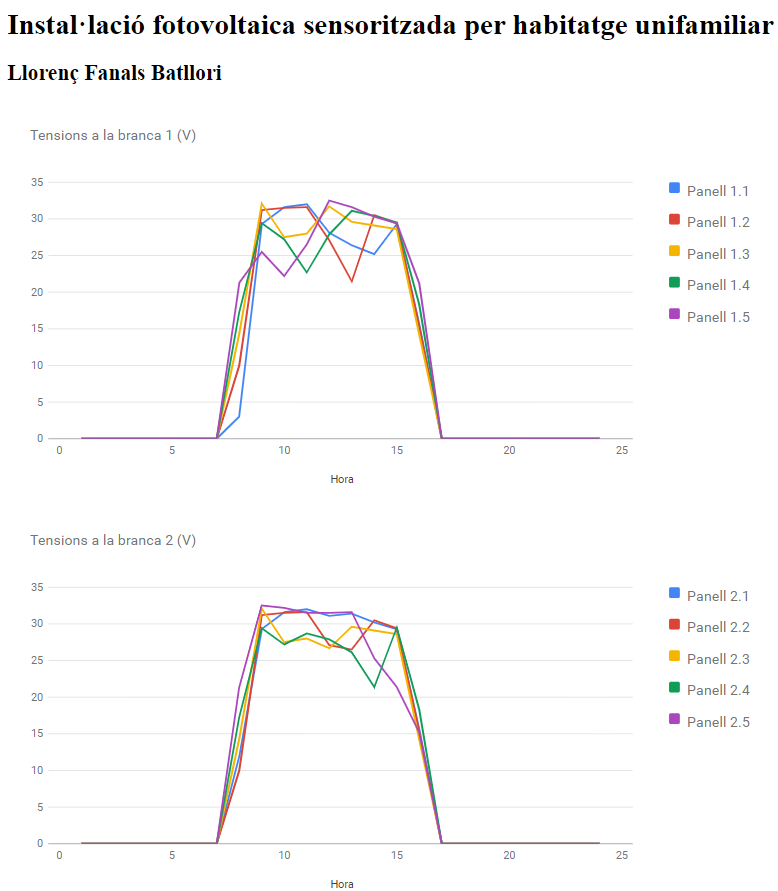
\includegraphics[scale=0.75]{images/c1.png}}
\end{center}
\caption{Part de la pàgina web}
\label{fig:1}
\end{figure}

\noindent \\ El fet d'utilitzar JavaScript permet inserir contingut dinàmic. Al passar el ratolí per sobre una línia es ressalta la línia i els punts que la formen. A la Figura \ref{fig:2} s'aprecia.
\begin{figure}[H]
\begin{center}
\fbox{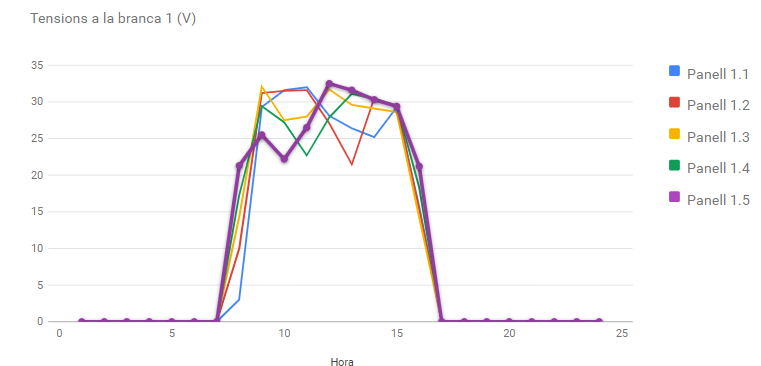
\includegraphics[scale=0.75]{images/c2.png}}
\end{center}
\caption{Gràfica d'un panell i punts ressaltats}
\label{fig:2}
\end{figure}

\noindent A més, és possible visualitzar el valor de cada punt col·locant el ratolí sobre seu, es veu a la Figura \ref{fig:3}.
\begin{figure}[H]
\begin{center}
\fbox{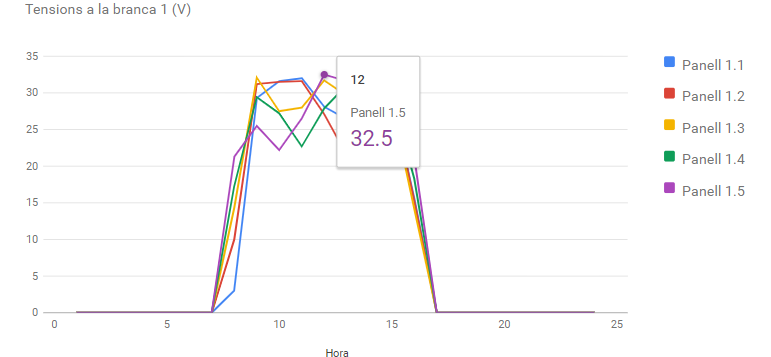
\includegraphics[scale=0.75]{images/c3.png}}
\end{center}
\caption{Gràfica d'un panell, lectura d'un dels seus punts}
\label{fig:3}
\end{figure}

\noindent A la pàgina web també s'ha inserit un croquis de la disposició de les plaques. Amb la imatge i les gràfiques el client pot deduir fàcilment quins panells estan més ombrejats, en quines hores i, en cas de tensions massa baixes, quins poden estar malmesos i necessiten ser revisats. Es mostra a la Figura \ref{fig:4}.

\begin{figure}[H]
\begin{center}
\fbox{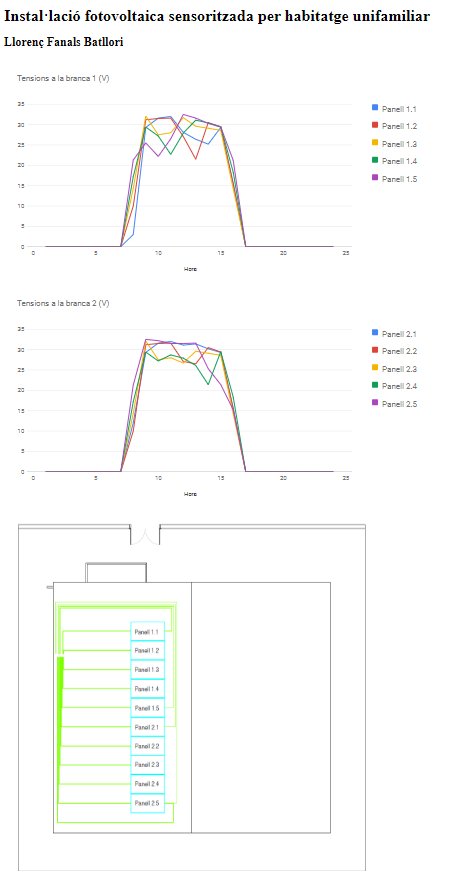
\includegraphics[scale=1.0]{images/c4.png}}
\end{center}
\caption{Pàgina web completa}
\label{fig:4}
\end{figure}





\clearpage


% Table generated by Excel2LaTeX from sheet 'Hoja1'
%\begin{table}[H]
%  \centering
%    \begin{tabularx} {\textwidth} {|X|r|} \hline
%  \multicolumn{1}{|c|}{Descripció} &  \multicolumn{1}{c|}{Quantitat}\\ \hline \hline
%
 %   Placa GLC 330 W & 10 \\ \hline
%    Inversor FRONIUS Primo 3.0-1 Light 3kW & 1 \\ \hline
%    Metres cable Ethernet RJ-45 CAT 8 & 10 \\ \hline
%    Metres cable 4 m$m^2$ PVC & 45 \\ \hline
 %   Metres cable 1,5 m$m^2$ PVC & 100 \\ \hline
 %   Punteres Enghofer E 4-10, 4 m$m^2$, 10 mm & 20 \\ \hline
 %   Punteres Enghofer E 1.5-10 1,5 m$m^2$ 10 mm & 12 \\ \hline
 %   Cinta aïllant 10 m 1,6 cm & 3 \\ \hline
 %   Caixa estanca Solera CONS 100x100x55 mm & 2 \\ \hline
  %  Canal Euroquint 25,16 mm 1,5 metres & 20 \\ \hline
%    Curva canal VECAMCO & 10 \\ \hline
%    Paquet de 50 brides 200x2,6  mm & 2 \\ \hline
%    Regleta nylon 12 pols 16 mm & 4 \\ \hline
%    Premsaestopes M12 & 10 \\ \hline
%    Cargol autoroscant M4 16 mm & 12 \\ \hline
%    Tacs Fischer 072095 nylon 6x50 mm & 50 \\ \hline
%    Díode SM74611KTTR & 10 \\ \hline
%            Hores enginyer & 1 \\ \hline
%    Hores oficial de primera & 12 \\ \hline
%    Hores oficial de segona & 12 \\ \hline
%    \end{tabularx}%
%  \label{tab:addlabel}%
% \end{table}%
